\documentclass{article}
\usepackage[fleqn]{amsmath}
\usepackage{amssymb,graphicx,color,graphicx,slashed, microtype, parskip, enumitem, extarrows, needspace}
%\usepackage[utf8x]{inputenc}
\usepackage[top=1.5cm, bottom=1.5cm, right=6cm, left=1.5cm, heightrounded, marginparwidth=5cm, marginparsep=0.5cm]{geometry}

\hbadness = 10000
\hfuzz=100pt 
    
\usepackage{marginnote}
\renewcommand*{\marginfont}{\footnotesize}

\usepackage{hyperref}
\hypersetup{colorlinks=true, urlcolor=NavyBlue, bookmarksdepth=3}

\makeatletter\newcommand{\@minipagerestore}{\setlength{\parskip}{\medskipamount}}\makeatother

% =============== Index ===========================

\usepackage[nonewpage]{imakeidx}
\makeindex

% =============== Color Definitions ===============
    
\usepackage[svgnames]{xcolor}
\colorlet{ColorTitle}{Black}
\colorlet{ColorSectionName}{Black}
\colorlet{ColorBoxFG}{Gray}
\colorlet{ColorBoxText}{Black}
\colorlet{ColorBoxBG}{White}


% =============== Title Style ===============
    
\usepackage{titling} % Allows custom title configuration
    
\newcommand{\HorRule}{\color{ColorTitle}\rule{\linewidth}{1pt}} % Defines the gold horizontal rule around the title
    
\pretitle{
    \vspace{-50pt} % Move the entire title section up
    \HorRule\vspace{9pt} % Horizontal rule before the title
    \fontsize{27}{36}\usefont{OT1}{phv}{b}{n}\selectfont
    \color{ColorTitle} % Text colour for the title and author(s)
}
    
\posttitle{\par\vskip 15pt} % Whitespace under the title
    
\preauthor{\fontsize{17}{0}\usefont{OT1}{phv}{m}{n}\selectfont\color{ColorTitle}} % Anything that will appear before \author is printed
    
\postauthor{\par\HorRule}

\newcommand{\COURSENAME}{\href{http://phyw.people.ust.hk/teaching/PHYS2022-2015/}{\textcolor{black}{PHYS 2022}}}
\newcommand{\YW}{\href{http://phyw.people.ust.hk/}{\textcolor{black}{Yi Wang}}}
\newcommand{\PHYS}{\href{http://physics.ust.hk}{\textcolor{black}{Department of Physics}}}
\newcommand{\HKUST}{\href{http://www.ust.hk/}{\textcolor{black}{HKUST}}}
\author{\COURSENAME, \YW, \PHYS, \HKUST}

\date{}

% =============== Section Name Style ===============
    
\usepackage{titlesec}
    
\titleformat{\section}
    {\fontsize{15}{20}\usefont{OT1}{phv}{b}{n}\color{ColorSectionName}}
    {\thesection}{1em}{}
    %[{\vspace{0.2cm}\titlerule[0.8pt]}]
    
\titleformat{\subsection}
    {\fontsize{14}{20}\usefont{OT1}{phv}{m}{n}\color{ColorSectionName}}
    {\thesubsection}{1em}{}
    
\titleformat{\subsubsection}
    {\fontsize{12}{20}\usefont{OT1}{phv}{m}{n}\color{ColorSectionName}}
    {}{0em}{}
      
\setcounter{secnumdepth}{4}
        
% =============== Box Style ===============
    
\usepackage[most]{tcolorbox}
    
\newtcolorbox{tbox}[1]{
    colback=ColorBoxBG, colframe=ColorBoxFG, coltext=ColorBoxText,
    sharp corners, enhanced, breakable, parbox=false,
    before skip=1em, after skip=1em,
    title={#1}, fonttitle=\usefont{OT1}{phv}{b}{n}, 
    attach boxed title to top left={yshift=-0.1mm}, boxed title style={sharp corners, colback=ColorBoxFG, left=0.405cm},
    rightrule=-1pt,toprule=-1pt, bottomrule=-1pt
}

\newtcolorbox{mtbox}[1]{
    colback=ColorBoxBG, colframe=ColorBoxFG, coltext=ColorBoxText,
    sharp corners, enhanced, breakable, parbox=false,
    before skip=1em, after skip=1em,
    title={#1}, fonttitle=\usefont{OT1}{phv}{b}{n},
    attach boxed title to top left={yshift=-0.1mm}, boxed title style={sharp corners, colback=ColorBoxFG, left=0.15cm},
    rightrule=-1pt,toprule=-1pt, bottomrule=-1pt, 
    left=0.5em
}

% =============== tikz has to be loaded after xcolor
\usepackage{tikz}

\newcommand*\enumlabel[1]{\tikz[baseline=(char.base)]{
			\node[shape=rectangle,inner sep=2pt,fill=ColorBoxFG] (char) 
			{\fontsize{7}{20}\usefont{OT1}{phv}{b}{n}{\textcolor{ColorBoxBG}{#1}}};}}

% =============== Useful shortcuts ===============

\newcommand\wref[1]{{\hypersetup{linkcolor=white}\ref{#1}}}  

\newcommand{\textbox}[2]{
    \begin{tbox}{#1}
        #2
    \end{tbox}
}

\newcommand{\mtextbox}[2]{\marginnote{
    \begin{mtbox}{#1}
        #2
    \end{mtbox}}
}

\newcommand{\mnewline}{\vspace{0.5em}\newline}

\newcommand{\titem}[1]{
    \begin{itemize}[label=\color{ColorBoxFG}$\blacktriangleright$, leftmargin=0mm, labelsep=0.27cm, topsep=0.5em
        %, itemsep=1ex
        ]
        #1
    \end{itemize}
}

\newcommand{\mtitem}[1]{
    \begin{itemize}[label={\color{ColorBoxFG}$\blacktriangleright$}, leftmargin=0mm, labelsep=1mm, topsep=0.5em
        %, itemsep=1ex
        ]
        #1
    \end{itemize}
}

\newcommand{\itembox}[3]{
    \begin{tbox}{#1}
        #2
        \titem{#3}
    \end{tbox}
}

\newcommand{\mitembox}[3]{
    \marginnote{
    \begin{mtbox}{#1}
        #2
        \mtitem{#3}
	\end{mtbox}
    }
}

\newcommand{\tenum}[1]{
    \begin{enumerate}[label=\protect\enumlabel{\arabic*}, leftmargin=0mm, labelsep=0.265cm, topsep=0.5em
        %, itemsep=1ex
        ]
        #1
    \end{enumerate}
}

\newcommand{\enumbox}[3]{
    \begin{tbox}{#1}
        #2
        \tenum{#3}
    \end{tbox}
}

\newcommand{\twocol}[5]{
    \begin{minipage}[t][][b]
        {#1\textwidth}
        #4        
    \end{minipage}
    \hspace{#2\textwidth}
    \begin{minipage}[t][][b]
        {#3\textwidth}
        #5
    \end{minipage}
}

\newcommand{\cg}[2]{
    \begin{center}
        \includegraphics[width=#1\textwidth]{#2}
    \end{center}
}

\newcommand{\tbar}{
    ~\newline
    {\color{ColorBoxFG}
    \hbox to 0.15\textwidth{\leaders\hbox to 5pt{\hss  \hss}\hfil} 
    \hbox to 0.7\textwidth{\leaders\hbox to 5pt{\hss . \hss}\hfil}}
    \mnewline
}

% =============== Filter unwanted warnings
\usepackage{silence}
\WarningsOff[tcolorbox]
\hbadness=1000000


\graphicspath{{7_fig/}}
\usepackage{ctex}
\title{第七章\ 从行为到 \\
自然法则}

\begin{document}

\maketitle

\mtextbox{运动方程}{
    用来推算粒子运动路径的一个关于时间的二次微分方程(或方程组)叫做运动方程。\index{运动方程}比如说,粒子在势 $V(q)$ 中的运动可以用运动方程$\ddot q + dV/dq = 0$来描述。解实际问题的时候,运动方程还包含了初始条件:初始时间$t_0$以及$q(t_0)$与$\dot q(t_0)$的值。求解具有这种初始条件的运动方程称为柯西问题。\index{柯西问题}.
}
\textbox{一种新的物理思维方式}{
    我们习惯用牛顿的方式思考物理--对于粒子来说,如果我们知道初始位置和速率,我们可以计算该粒子一段时间的路径。这种思维方式可以推广到重力、电磁场、及其他概念上。

    但是如果我们真的想要思考基础的问题--这些运动方程能否成为自然的终极密码——仍然有一些不完美的方面:
    
     \tenum{
        \item 运动方程在狭义相对论中不是不变的对象,因为运动方程是时间演化的。在相对论中,时间和空间有几乎相同的权力。对于不同的观测者,运动方程是(以洛伦兹变换)协变,而非不变。自然的终极密码真的那么主观吗?在电影黑客帝国中,整个世界都是一个程序。那些程序员是否在这部电影中只选择了一个喜欢的帧来写下运动方程并对世界进行编码?
        \item 那些守恒定律是从哪里来的?我们知道能量、动量、角动量、电荷守恒定律。在特定的理论框架下,我们可以证明它们。比如说,在牛顿力学的框架下,我们可以运用聪明的技巧来证明能量和动量守恒。但是是否存在一个通用方法来找出所有系统的守恒定律的起源?
        \item 受限运动。比如说,想象一个钟摆(如果太简单,想象两个)。
        理想理论下,受限运动意味着我们减少了运动的可能性,从而使情况更简单。但是在牛顿物理中,越多限制意味着越多力的分析与更复杂的数学。有没有一种方法可以让受限系统更方便计算呢?
        \item 量子世界与与之对应的经典世界有很大的不同。我们还没有介绍量子力学,但是之后我们会解决这个问题。
        \item 这些运动方程对于解释自然的“习性”来说太“冷血”了。你可以用一句话概括自然法则(适用于所有已知基础物理)吗?比如说,“自然一般会$\cdots$”?仅仅说自然一般会满足运动方程似乎不足够信服别人。 
    }
    \tcblower
    莫佩尔蒂(1698-1759)说的一个短句很好地解决了以上问题:

    “自然的一切行为都是最简洁的。” \index{最小作用量原理}

    我们将看到这个简单的句子是如何工作的。
}

\section{费马原理}\label{sec:fermat}

在解决最小作用量原理之前,我们先用费马原理\index{费马原理}来研究光的传播。这还不是真正的最小作用量原理,但是它的物理概念和数学方法是极其相似的。它也是非常直观的,所以我们先做一个热身练习。

\mtextbox{皮埃尔·德·费马}{
    皮埃尔·德·费马(1601或1607 - 1665)是一个法国律师。不过没人记得他为什么案子辩护过。我们只记得他的一些其他事情,例如他对于$n>2$,$x^n+y^n=z^n$ 没有正整数解的猜想。直到300年后,这个猜想才在1994年被证明。
}
\textbox{费马原理}{
    \twocol{0.3}{0.05}{0.65}{
        考虑一类光传播的问题:已知两个定点$P$和$Q$,光是如何在两点之间传播的?
    
    右图给了可用空间的传播、反射、折射的例子。
    }{
        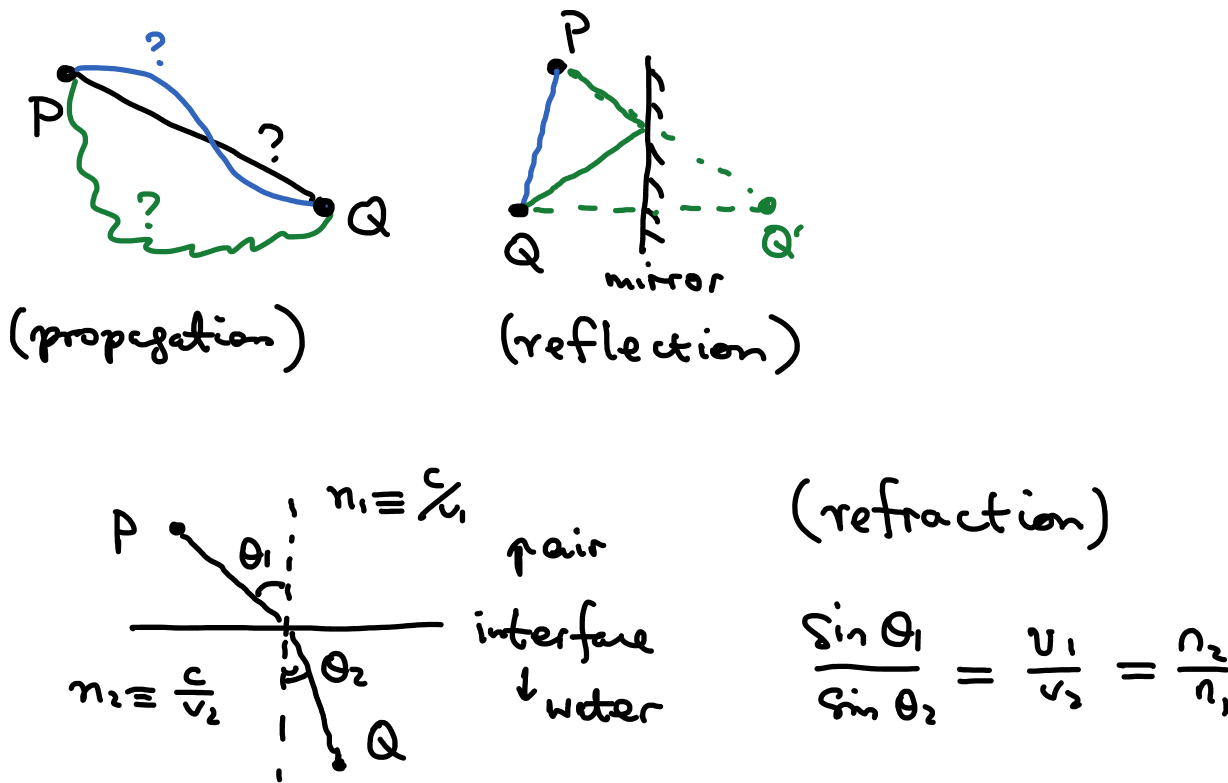
\includegraphics[width=\textwidth]{fermat}   
    }

    \tcblower

    费马提出了一个对这种问题的通用答案:光沿着极值时间的路径在两个已知点之间传播。
}

\textbox{行动时间如何取决于路径?泛函}{
    我们在微积分中熟知了极限问题:一个函数$f(x)$在$df/dx=0$时取极限值。我们这里的情况很相似,只不过使用不同的数学对象..

    \marginnote{当然并不是所有路径都可以被$y=y(x)$参数化,比如说x为常数。这里我们只关注可以被$y=y(x)$参数化的路径,因为它们可以提供足够的背景来推导最小作用量原理。}
    我们说的是空间(数学意义)的“路径”。怎么在数学中参数化一个路径呢?一个路径可以被看成一个函数。比如说,一个曲线$y=y(x)$。

    假设我们知道光速(真空中为$c$,在折射率$n$ 的介质中为$c/n$)。已知一个路径,我们可得光的传播时间$T$。这里的$T$取决于整个函数$y$(而不是$y(x)$在不同$x$时候的值)。我们可以说$T$是一个$y$的\emph{泛函},写做$T[y]$。
    
    长话短说,泛函是一个“函数的函数”。\index{泛函} 下图显示了函数和泛函的对比。

    \mtextbox{函数式编程}{在编程语言中,有个典范叫函数编程。它最基本的要求是你可以将函数作为另一个函数的参数传递。它与泛函一样(都是函数的函数)。}

    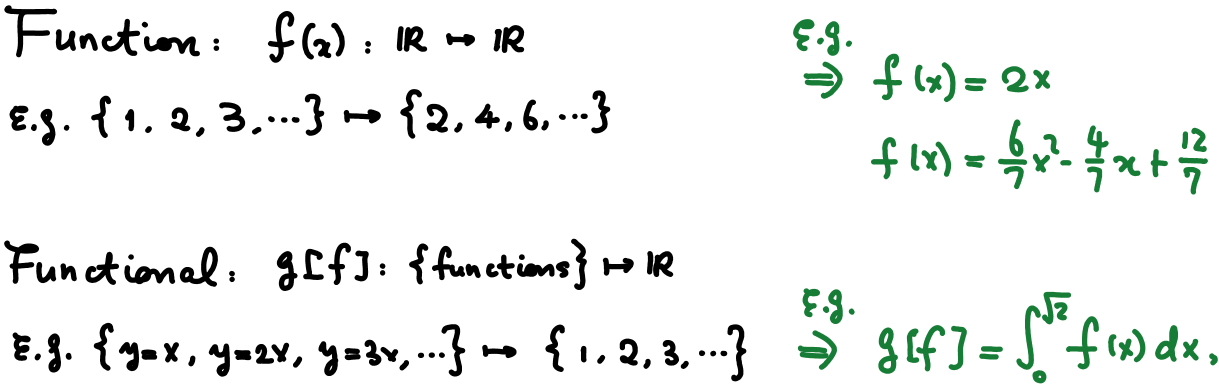
\includegraphics[width=0.8\textwidth]{functional}
}

\needspace{0.15\textheight}
\marginnote{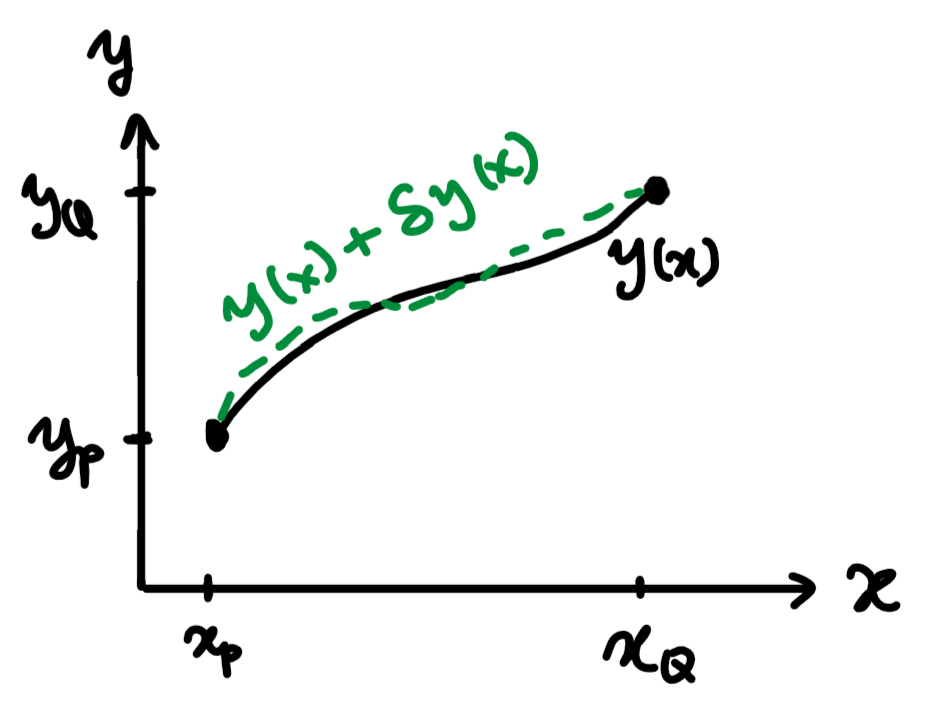
\includegraphics[width=0.3\textwidth]{variationyx}}
\textbox{哪个路径有极限时间?变分法\index{变分法}}{
    为了求$(x_P, y_P)$与$(x_Q, y_Q)$的极限时间,我们先画一个(通用)满足$y(x_P)=y_P$和$y(x_Q)=y_Q$的路径$y(x)$。然后我们找一些极限路径必须满足的条件。运用以下步骤:
    
    我们通过$y(x) \rightarrow y(x)+\delta y(x)$改变路径。$\delta y$为\emph{任意}无穷小函数(即我们可以忽略$(\delta y)^2$) 且满足$\delta y(x_P)=0$和$\delta y(x_Q)=0$。这些“边界条件”需要被满足,因为根据问题的定义,我们已经确定了这两个边界点。

    那么现在新路径的时间为$T[y+\delta y]$,泛函为
    \begin{align}
        \delta T \equiv T[y+\delta y] - T[y]~.
    \end{align}
    \mtextbox{为什么$\delta T=0$代表了极值?}{原因与在微积分里为什么函数$y(x)$在 $dy/dx=0$的时候有极值很相似。假设这个极值是一个局部最小值。考虑$y(x)$在$(x, x+dx)$之间的变化,保持在这个区域外的固定(这是 $\delta y$一种允许的形式)。那么如果$\delta T\neq 0$在$(x, x+dx)$之间,变化$\delta T = (\cdots) \delta y dx$。如果$(\cdots)$是负数,变化$\delta y$让$T$更小。那么$T$就不是最小值。如果$(\cdots)$是正数,那么变化$-\delta y$让$T$更小。那么$T$仍然不是最小值。因此,对于最小的 $T$,$\delta T$ 在 $(x, x+dx)$ 内消失。由于 $(x, x+dx)$ 是一个区间,$\delta T$ 应该在任何地方都消失。 局部最大值的证明同理。}
    对于所有可能的变化$\delta y(x)$,极值时间的路径一定满足$\delta T = 0$。
}

以上可能看着很枯燥和空洞。那么我们来看一个例子。

\textbox{真空中光的传播}{
    我们研究的光在$(x_P, y_P)$与$(x_Q, y_Q)$之间自由传播。假设我们只知道费马定理和光速为$c$。为了简单来说,我们抑制了$z$方向。我们只研究$x,y$空间维度。两点之间的传播时间$T$可以写为
    \begin{align}
        T = \int_{t_P}^{t_Q} dt 
        = \frac{1}{c} \int_{x=x_P, y=y_P}^{x=x_Q, y=y_Q} \sqrt{dx^2 + dy^2}
        = 
        \frac{1}{c} \int_{x_P}^{x_Q} \sqrt{1 + \left(\frac{dy}{dx}\right)^2 } ~ dx ~.    
    \end{align}
    为了找到极限路径$y(x)$必须满足的条件,我们改变 $y(x)\rightarrow y(x)+\delta y(x)$并带入以上等式。因为 $d\delta y / dx$非常小,我们可以当它是一个极小参数并进行泰勒展开:
    \begin{align}
        \label{eq:integrand}
        \sqrt{1 + \left(\frac{d[y(x)+\delta y(x)]}{dx}\right)^2 }
        = \sqrt{1+(y')^2} + 
        \frac{y'}{\sqrt{1+(y')^2}} \frac{d \delta y}{dx} + \mathcal{O}[(\delta y)^2]~, 
      \end{align}
      这里$y'\equiv dy(x)/dx$。因此
      \begin{align}
        \label{eq:Tvariation}
        \delta T[y] & = \frac{1}{c} \int_{x_P}^{x_Q}
        \frac{y'}{\sqrt{1+(y')^2}} \frac{d \delta y}{dx} ~ dx \nonumber\\ &
        = \frac{1}{c} \int_{x_P}^{x_Q} \left\{
        \frac{d}{dx} \left ( \frac{y'}{\sqrt{1+(y')^2}} \delta y \right ) 
        - \delta y \frac{d}{dx} \left ( \frac{y'}{\sqrt{1+(y')^2}} \right ) \right\} 
        ~ dx \nonumber\\ &
        = - \frac{1}{c} \int_{x_P}^{x_Q} 
        \delta y \frac{d}{dx} \left ( \frac{y'}{\sqrt{1+(y')^2}} \right )  
        ~ dx~,
      \end{align}  
      这里我们完全忽略了导数项因为$\delta y=0$在边界上。

      $\delta T=0$需要使以上等式对于所有$\delta y$都消失。因此我们需要满足
      \begin{align}
        \label{eq:yvariation}
        \frac{d}{dx} \left ( \frac{y'}{\sqrt{1+(y')^2}} \right) = 0
        \quad\rightarrow\quad
        y'=\mbox{const}~.
      \end{align}
      我们就证明了费马定理中的光沿直线运动。
}

通过更多的努力,我们可以通过费马定理及一些变形式推算出反射、折射的光的路径。但是这里我们不会做。

这里我们是在运用很复杂的方法来做一个很简单的事情。但是这里提出的技术(数学)会在关于运动定理的下节被重新运用。

\section{Principle of Extremal Action}

One may live a life in two ways: (1) Given the current state, this is what I'd like to do now. And I will evolve with time and see what future will become; and (2) Given the current state, I have a clear dream of my future. And I will find out the master plan where my dream can come true.

Interestingly, physics can also be understood in these two ways (and they are equivalent): (1) corresponds to the Cauchy problem -- solving the equation of motion with initial position and velocity; and (2) corresponds to the action principle, which we are now to introduce.

\textbox{The action principle \index{action principle}}{
    A theory is defined by an action $S$. The equation of motion of the theory corresponds to the extremal action $\delta S = 0$.
}

Let us first see how this works in Newtonian mechanics. Later we generalize it to include all known fundamental theories.

\marginnote{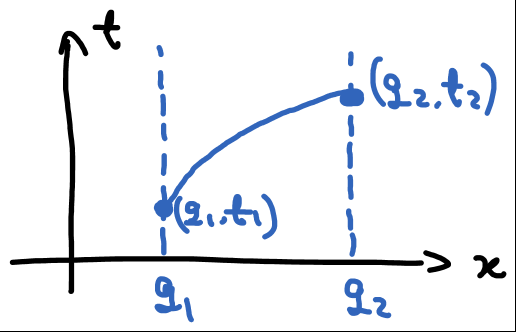
\includegraphics[width=0.3\textwidth, trim={0 2pt 2pt 0}, clip]{newton}}
\textbox{Action principle in Newtonian mechanics}{\index{action of Newtonian mechanics}
    Newtonian mechanics can be formulated as the following question: 

    Given a potential $V(q)$, where $q(t)$ is the position of the particle, what is the trajectory between a starting point $(q_1, t_1)$ and a final point $(q_2, t_2)$?

    First let us define an action
    \mtextbox{A remark on integral convention}{Physicists sometimes write $\int dt f(t)$. This is identical to $\int f(t) dt$. It is just a matter of notation. But it reflects that physicists tend to think an integral as a limit of summation: $\lim_{\Delta t\rightarrow 0} \sum_i \Delta t f(t_i) = \int dt f(t)$. Here $\Delta t$ and $f(t_i)$ are just multiplied together and thus the order is not important.}
    \begin{align}
    \label{eq:newtonAction}
    S[q] = \int_{t_1}^{t_2} dt \left [ 
    \frac{1}{2} m \dot q ^2 - V(q)
    \right ]~.
    \end{align} 
    The action has a form of integrating $K-V$ over time, where $K$ is the kinetic energy and $V$ is the potential energy. This is quite general. Do not ask about the physical meaning at the moment. We just define such a functional (functional of paths $q(t)$) and see what it leads to. We will come back to its physical meaning (and also why the extremal action principle at all) in Section \ref{sec:action-quantum}.

    To derive the equation of motion, similarly to Section \ref{sec:fermat}, we vary $q(t)\rightarrow q(t)+\delta q(t)$, which satisfies $\delta q(t_1)=\delta q(t_2) = 0$, and see how the action changes:
    \mtextbox{Motion with constraints}{By now, you should be able to solve the motion with constraints, for example, double pendulum in a smarter way than Newtonian analysis of forces. As an exercise, you may use two angles to parameterize $K$ and $V$ of the system and write $S=\int dt (K-V)$. Variation principle gives you much simpler result than what you would have calaulated using forces.}
    \begin{align}
        \label{eq:dSNewton}
        \delta S = \int_{t_1}^{t_2} dt 
        \left [ m \dot q \delta \dot q - \frac{dV}{dq} \delta q   \right ]
        = \int_{t_1}^{t_2} dt 
        \left [ \frac{d}{dt}(m\dot q \delta q) - m\ddot q \delta q - \frac{dV}{dq}\delta q  \right ]~.
    \end{align} 
    Again the first term is a boundary term that vanishes. The last two terms holds for all $\delta q(t)$ and thus we have re-derived Newtonian equation of motion for a particle:
    \begin{align}
        \label{eq:eomNewton}
        m\ddot q + \frac{dV}{dq} =0~.
    \end{align}
}

\needspace{0.15\textheight}
\mtextbox{Math of the Lagrangian}{By writing $L=L(q_i, \dot q_i, t)$, it is in the sense of multi-variable calculus: one can calculate partial derivatives on the three variables ``independently'' assuming the rest two variables do not change. For example, $\partial_t L \equiv \partial L / \partial t$ assumes that $q_i$ and $\dot q_i$ do not change when calculating the partial derivative. This is different from 
\newline$dL/dt$ $= \sum_i (\partial L / \partial q_i)(dq_i/dt)$ 
\newline$+ \sum_i (\partial L / \partial \dot q_i) (d\dot q_i/dt)$ $+ \partial L / \partial t$. }
\textbox{A General action and the Euler-Lagrange equation}{\index{Euler-Lagrange equation}
    In general, consider a ``Lagrangian''\index{Lagrangian} $L=L(q_i, \dot q_i, t)$, where $i=1, 2, \ldots, N$. Here $q_i$ denotes the position of the $i$-th particle. (In fact, in the spirit of general coordinate, the index $i$ can also collectively denote many possible things: different spatial dimensions, different particles, values of fields at a point, and so on. We will not dive into those details.)

    The action is defined as
    \begin{align}
        \label{eq:actionL}
        S = \int L(q_i, \dot q_i, t) dt~.
    \end{align}
    Here we have not written down the limits of the integral, having in mind that the boundary terms will be dropped. Clearly, this definition includes the Newtonian particle example that we have studied, and is much more general.

    The equation of motion of such a general system, known as the Euler-Lagrangian equation, can be derived by the variation
    \mtextbox{Dropping the boundary temrs}{
        From now on we will assume that the boundary terms $\int \partial_t(\cdots) dt$ can be dropped. The argument is that this term does not modify the EoM. A careful treatment of the boundary terms is beyond the scope of this lecture; but dropping these boundary terms doesn't hurt for all our current purposes. 
    }
    \begin{align}
    \label{eq:dSEL}
    \delta S & = \sum_i \int \left ( 
    \frac{\partial L}{\partial \dot q_i} \delta\dot q_i  
    + \frac{\partial L}{\partial q_i} \delta q_i 
    \right ) dt \nonumber\\ &
    = \sum_i \int \left [
        \frac{d}{dt} \left ( \frac{\partial L}{\partial\dot q_i} \delta q_i \right )
        -  \frac{d}{dt} \left ( \frac{\partial L}{\partial\dot q_i} \right)\delta q_i
        + \frac{\partial L}{\partial q_i} \delta q_i
    \right ] dt~.
    \end{align}
    Thus the Euler-Lagrangian equation (holds for every $i$) can be read off as
    \begin{align}
    \label{eq:eomEL}
    \frac{d}{dt} \left ( \frac{\partial L}{\partial\dot q_i} \right)
    - \frac{\partial L}{\partial q_i} = 0 ~.
    \end{align}
}

\textbox{All known fundamental physics in one line}{
    All known fundamental physics can be written into an action\index{action of the Standard Model}
        \begin{align}
          \label{eq:SMaction}
          S \sim \int d^4 x \sqrt{-g} \Big\{ 
          \frac{1}{16\pi G}  R 
          - \frac{1}{4} F^2 
          + i \bar\psi \slashed{D} \psi 
          + |D h|^2 - V(h) 
          + h \bar\psi \psi 
          \Big\}~.
        \end{align}
    This action covers the laws of gravity (the metric $g$), E\&M and their friends (gauge field in $F$), electrons and their friends (spinor fields represented by $\psi$) and origin of mass (the Higgs field $h$). These fields, put together with certain gauge symmetries, is known as the particle physics Standard Model and describes all known fundamental physics.
    We shall not explain it here (a course of particle physics or quantum field theory needed). Take it as a piece of art at the moment.
    }

\section{Symmetry and Conservation Laws}

In the part of special relativity, at relativistic momentum and energy, we have argued why we need conservation laws: (1) physically, allow us to ignore the details happened in the middle; (2) mathematically, reduce 2nd order ODEs into 1st order or 0th order; (3) provide observables for modern physics. 

But the question left is, why there exists conservation laws after all? To ask the question in general, we had better to use a universal framework of physical theories to find the root of conservation laws. Thus the general action \eqref{eq:actionL} is a good starting point.

Instead of directly asking why anything is conserved in \eqref{eq:actionL}, let's first think about a piece of beauty -- symmetry of a theory.

\needspace{0.2\textheight}
\mtextbox{Remarks about symmetry}{
    \mtitem{
        \item The action is a means to derive equations of motion. Thus to examine the change of the action under \eqref{eq:sym-trans-q}, any equation of motion must not be used (to avoid circular arguments). To be explicit, when talking about $\delta S=0$, we may mean one of the two things: (1) a symmetry transformation without using equation of motion; or (2) any transformation (may not be a symmetry) as a variation principle, and use the equation of motion. One should be clear about the difference.
        \item Again we assume to drop boundary terms $\int \partial_t (\cdots) dt$ when considering the change of the action. This is to say, if the Lagrangian $L(\tilde q_i, \dot {\tilde q}_i, t) \neq L(q_i, \dot q_i, t)$, but rather $L(\tilde q_i, \dot {\tilde q}_i, t) = L(q_i, \dot q_i, t) - \epsilon dg/dt$ for arbitrary $g$, the transformation is still considered a symmetry.
        \item As $\epsilon$ is infinitesimal, we will ignore the $\mathcal{O}(\epsilon^2)$ terms.
        \item The type of symmetry \eqref{eq:sym-trans-q} that we study here is a continuous and global symmetry. There are other types of symmetries, namely discrete symmetries and gauge symmetries, which will not be useful to derive nontrivial conservation laws.
    }
}
\textbox{A symmetry of a theory}{\index{symmetry}
    A symmetry of a theory is a transformation under which the theory does not change.
    \tcblower
    In terms of \eqref{eq:actionL}, the above definition of symmetry can be put more explicitly as: 
    
    Consider an infinitesimal transformation\index{transformation}
    \begin{align}
        \label{eq:sym-trans-q}
        q_i \rightarrow \tilde q_i = q_i + \epsilon \delta q_i~,
    \end{align}
    where $\epsilon$ is an infinitesimal constant. If the action does not change
    \begin{align}
        \label{eq:sim-trans-s}
        \delta S = \int L(\tilde q_i, \dot {\tilde q}_i, t) dt - \int L(q_i, \dot q_i, t) dt = 0 ~,
    \end{align}
    then we consider the transformation \eqref{eq:sym-trans-q} a symmetry.
}
The definitions \eqref{eq:sym-trans-q} and \eqref{eq:sim-trans-s} are very abstract. We thus consider a few examples:
\textbox{Examples of transformations}{
    \titem{
        \item Time translation\index{time translation}, to test if the prediction of a theory is time dependent. The transformation thus relate two situations: doing an experiment now and doing an experiment a bit later (within the same theory) and observe if there is any difference. The time translation can thus be written as
        \begin{align}
            q_i (t) \rightarrow \tilde q_i(t) = q_i (t + \epsilon \delta t) 
            = q_i (t) + \epsilon \dot q_i(t) \delta t~.
        \end{align}
        We thus extract that for time translation
        \begin{align}
            \delta q_i = \dot q_i(t) \delta t~.
        \end{align}
        We will later study the consequence of time translation in great detail in this section.
        
        \marginnote{For space translation, is $\delta q_i$ the same for different $i$? We will need to examine what $i$ actually means then: If $i$ stands for diffferent directions in space, then $\delta q_i$ can take different values. If $i$ stands for different particles in the same direction, then $\delta q_i$ must take the same value for different $i$.}
        \item Space translation, to test if doing an experiment in one place is identical to doing an experiment in a slightly different location. The transformation is thus $q_i(t) \rightarrow q_i (t) + \epsilon \delta q_i$, where $q_i$ is a constant shift. The space translation can be related to momentum conservation.

        \item Lorentz transformation. The boost between $(t_B, x_B)$ and $(t_A, x_A)$ for infinitesimal $\beta$ (or rotation). When $\beta$ is small, $\gamma\approx 1$. Then approximately $t_B \simeq t_A + \epsilon v x_A/c^2$, $x_B \simeq x_A + \epsilon v t_A$. We thus have $q_i(t) \rightarrow q_i (t+ \epsilon v q_i /c^2) + \epsilon v t$ This boost part can be related to (not very interestingly) the initial center of energy. The rotation part of Lorentz transformation can be defined similarly and is related to angular momentum conservation

        \item Change of phase. If $q_i$ are complex, it makes sense to examine the transformation $q_i \rightarrow e^{i \epsilon \alpha} q_i$. This can be related to charge conservation. 
    }
}

We have studied many transformations. Let's move on to explore the requirement for a transformation to be a symmetry. We only take time translation as an example.
\textbox{When is time translation a symmetry?}{
    \marginnote{Note that $L=L(q_i, \dot q_i)$ is a sufficient condition of time translation symmetry, but not a necessary condition. We will not explore the necessary condition here.}
    Intuitively, if the theory as specified by the Lagrangian $L$ does not explicitly depend on $t$ (i.e. $L(q_i, \dot q_i,t)=L(q_i, \dot q_i)$, without explicit $t$ dependence), the theory is time translation invariant. Here we will test that in this case, the time translation is indeed a symmetry.
    \tcblower
    Under time translation, considering that $\epsilon$ is a constant, we have
    \begin{align}
        \delta q_i = \dot q_i \delta t~, \qquad \delta \dot q_i = \ddot q_i \delta t~.
    \end{align}
    \begin{align}\label{eq:dL-time-translation}
        \delta L = L(q_i + \epsilon \dot q_i \delta t, \dot q_i + \epsilon \ddot q_i \delta t) 
        - L(q_i, \dot q_i)
        = \left [
            \frac{\partial L}{\partial q_i} \dot q_i 
            + \frac{\partial L}{\partial \dot q_i} \ddot q_i 
        \right ] \epsilon \delta t
        = \epsilon \frac{d( L \delta t)}{dt} ~.
    \end{align}
    When $\epsilon$ is a constant (as we already defined), this is indeed a symmetry. To see that, note that a total derivative is a boundary term (which we neglect) in the action. Thus \eqref{eq:sim-trans-s} holds.
}

We have inserted examples above to make things not too dry. But now let us back to very general discussions following equations \eqref{eq:sym-trans-q} and \eqref{eq:sim-trans-s}. They are not limited to time translation but in general for any symmetry.

\mtextbox{When can EoM be used}{
    We did not allow to use the equations of motion (EoM) when testing if a transformation a symmetry. But now, for requiring a conserved quantity to conserve, the equation of motion can indeed be used. For example, energy conservation indeed needs Newton's 2nd law (or relativistic generalizations) to apply. If a particle accelerates freely as it likes, it does not conserve energy.
}
\textbox{Conservation laws from symmetries\index{Noether theorem}}{
    Bear with me a mathematical trick: We have defined $\epsilon$ as a constant. Now, let's vary it: $\epsilon = \epsilon(t)$. A symmetry transformation keeps the action invariant when $\epsilon=$ const. Now how it should change when $\epsilon = \epsilon(t)$? The change of action should now take the form
    \begin{align}\label{eq:var-s-et}
        \delta S = \int (P \epsilon + Q \dot \epsilon) dt = \int Q \dot \epsilon dt = - \int \dot Q \epsilon dt + \mbox{(neglected boundary terms)}~. 
    \end{align}
    Here the $P$ term vanishes because a symmetry requires this term to vanish when taking $\epsilon=$ const. There are no terms such as $\ddot \epsilon$ because $L=L(q,\dot q, t)$ and there is no $\ddot q$ to generate $\ddot \epsilon$. At the last step integration by parts is used.

    \marginnote{If you really want to be careful about the boundary terms of the action, here you can choose $\epsilon(t)$ being a function that vanishes on the initial and final boundaries and thus we can indeed get rid of boundary terms.}
    \tcblower
    Now we are ready to interpret the physical meaning of \eqref{eq:var-s-et}. If we allow to use equations of motion, that is to say, $\delta S=0$ for all possible $\epsilon(t)$ (not because of a symmetry, but because of the action principle). Thus we have $\dot Q = 0$. In other words, $Q$ is a conserved quantity when equations of motion are used.

    This correspondence between a symmetry and a conserved quantity is known as the Noether's theorem.
}

In the above, we have shown the existence of a conserved quantity without showing actually what it is. This is not our style (unless you are a mathematician). What is the form of a conserved quantity given $L$ and $\delta q$?

\textbox{What is the conserved quantity in general?\index{conserved quantity}}{
    We have shown that, a symmetry leaves the action invariant and thus change the Lagrangian by at most a total derivative: $\delta L = - \epsilon dg/dt$ for some quantity $g$. When $\epsilon=\epsilon(t)$, we cannot drop this term. Also, the change of allowing $\epsilon = \epsilon(t)$ adds a term in the following step:
    \begin{align}
        \delta L = \sum_i \left[ 
            \frac{\partial L}{\partial q_i} \epsilon \delta q_i 
            + \frac{\partial L}{\partial \dot q_i} \partial_t (\epsilon \delta q_i) 
            \right]
            \supset
            \sum_i \frac{\partial L}{\partial \dot q_i} \delta q_i \dot\epsilon~. 
    \end{align}
    They are all the new terms that $\epsilon = \epsilon(t)$ brings and thus
    \begin{align}
        \delta S = \int \left ( g +  \sum_i \frac{\partial L}{\partial \dot q_i} \delta q_i \right )
        \dot \epsilon dt ~,
    \end{align}
    where we have performed an integration by part to the $g$-term. Compare with \eqref{eq:var-s-et}, we have the conserved quantity
    \begin{align}\label{eq:noether-charge}
        Q = g +  \sum_i \frac{\partial L}{\partial \dot q_i} \delta q_i ~.
    \end{align}
    When the equation of motion is used, $\dot Q = 0$ (conservation law). 
}

What is \eqref{eq:noether-charge}? It differs symmetry by symmetry. Let's see one example: time translation in Newtonian mechanics.

\mtextbox{When is conservation broken?}{The Noether theorem does not only tell what is the conserved quantity, but also tell explicitly the quantity is conserved under which situation. In the past we state that in an isolated system energy is conserved. Now we know that 
\mtitem{
    \item The condition can be relaxed: even the system is not isolated, as long as the time translation symmetry is not broken by the environment, energy is still conserved. (For example, in the case with a fixed gravitational potential, consider the source of gravity, such as the earth to be outside the system.)
    \item If the system is time-dependent, even if the system is isolated, energy may not be conserved. An example is our expanding universe.
}}
\textbox{Example: energy conservation as a result of time translation symmetry\index{energy conservation}}{
    Under time translation, the change of Lagrangian is \eqref{eq:dL-time-translation}. Thus, $g=-L\delta t$. The conserved quantity is the ``Hamiltonian''\index{Hamiltonian}
    \begin{align}
        H \equiv \frac{Q}{\delta t} = \sum_i \frac{\partial L}{\partial \dot q_i} \dot q_i - L~.
    \end{align}
    
    What's this? Consider more explicitly
    \begin{align}
        L = \sum_i \frac{1}{2} \dot q_i^2 - V(q_1, \ldots, q_n)~.
    \end{align}
    The conserved quantity is thus
    \begin{align}
        H = \sum_i \frac{1}{2} \dot q_i^2 + V~.
    \end{align}
    This conserved Hamiltonian is indeed the energy of the system.
}


\section{The Hidden Quantum Reality} \label{sec:action-quantum}

\textbox{The nature seems ``strange''}{
   The action principle offers a new way of thinking about how physics works. Take for example the motion of a particle moving from $A$ to $B$ in a force field:
   \marginnote{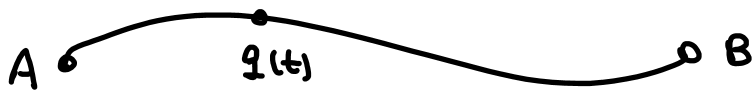
\includegraphics[width=0.35\textwidth]{question_action_newton}}
   \titem{
       \item Newton's view: The initial position and velocity are given. At each moment, the particle ``feels'' the force and ``adjusts'' its velocity according to the force. The adjusted velocity ``tells'' the particle how to move further.
       \item The action principle: The starting and end points are fixed, the particle needs to ``find'' its way between these two points based on an extremal action.
   }
   Do you feel the action way ``stranger''? It's straightforward for a particle to ``adjust'' its velocity in a force field (Newton's view). However, a particle cannot calculate (seriously in the theory of computation, since it may not even carry a bit of information or complicated enough for being even one logical gate). So how a particle can actually ``follow'' the action principle?

   Moreover, as we argued the action principle is a more fundamental way to describe all laws of nature. Why nature behaves fundamentally in such a ``strange'' way?
}

\textbox{The nature is natural but quantum\index{path integral}}{
    No. 
    \marginnote{You may think about a similar question: Why in a circuit, the electric current ``knows'' which way to go to minimize power? No, the current doesn't know. Rather, the electric field build up all possible paths until reach a stationary situation. More obvious examples include why flood ``knows'' where to flow, and so on. Definitely they are classical. But a particle can rely on its quantum nature to achieve a similar feature.}
    The nature is not strange. The nature is natural, but just not classical.
    
    Let's return to the question of the particle motion. Instead of ``calculating'' the extremal action, what the particle actually does is that, it ``tries'' \emph{all possible paths} and ``take'' the extremal one. 

    \tcblower

    The above words are actually nothing but the path integral formulation of quantum mechanics. In quantum mechanics, the probability $P$ for things to happen (here: particle to propagate from $A$ to $B$) is decomposed as
    \begin{align}
        P = |\mathcal{A}|^2~,
    \end{align} 
    where the complex number $\mathcal{A}$ is known as the probability amplitude. The probability amplitude can be calculated by a weighted average over all paths
    \begin{align}
        \mathcal{A} \propto \sum_{\small \mbox{all paths}} e^{iS/\hbar} ~.
    \end{align}
    Here by ``all paths'' we mean all possible lines connecting $A$ and $B$, not necessarily satisfy the equation of motion.
}

\mtextbox{What if $S\sim \hbar$?} {What about $S \sim \hbar = 1.05\times 10^{-34}$ $\mbox{m}^2$kg/s? Let us jump into the brave new world of quantum mechanics to answer this question in the next part! But in fact, we will use different but equivalent formulations of quantum mechanics (mainly wave mechanics and a bit of matrix mechanics) instead of the path integral. This is because the path integral, though conceptually simple, is harder in many computations. It will be included in a full quantum mechanics course. }
\textbox{The action principle explained\index{from quantum to classical}}{
    In the quantum world, the physical meaning of the action is clear: $e^{iS/\hbar}$ is the phase factor as a weight of the path in the summation of all paths.
    
    You may be confused here: in classical mechanics, the particle only select one trajectory. In quantum mechanics (path integral formulation), the particle move along all possible paths together. How to reconcile the difference? How the classical trajectory emerge among the quantum trajectories?

    \tcblower

    Classical mechanics emerges from quantum mechanics when $S\gg \hbar$. In this limit, even a very small change in $S$ (due to choosing a nearby different trajectory) results in a large change in the unit $\hbar$, and thus $e^{iS/\hbar}$ is a fast oscillating function, which cancels contributions of different paths almost for all paths.

    There is only one exception: close to the stationary action $\delta S=0$. Near $\delta S=0$ different paths do not cancel. Thus the classical trajectory is the only trajectory left over when the classical limit $S\gg \hbar$ is taken.
}

\section{Epilogue: Summary and What's Next}

\textbox{Further reading about the content}{
    \titem{
        \item Similar contents in other textbooks: You can find an extensive discussion of the content here in Part II of \href{https://www.amazon.com/Einstein-Gravity-Nutshell-Zee/dp/069114558X}{Einstein Gravity in a Nutshell} by Zee. You may also read the first section and the final appendix of \href{
            http://www.damtp.cam.ac.uk/user/db275/concepts/Concepts.pdf}{Lecture Notes on Modern Physics} by Baumann. 
        \item If you want even more references, I recommend to watch \href{
            http://theoreticalminimum.com/}{Theoretical Minimum (Video Lectures)}  (Lectures 3 and 4 of Classical Mechanics) by Susskind; or to read Chapter 2 of \href{https://www.amazon.com/Classical-Mechanics-3rd-Herbert-Goldstein/dp/0201657023}{Classical Mechanics} by Goldstein, Poole Jr and Safko. 
    }
}

\textbox{What happens next in a university physics program?}{
    \titem{
        \item Classical mechanics. The action principle is closely related to the Lagrangian formulation of classical mechanics. There is also a Hamiltonian formulation. You will see how mechanics are written in these ways. You will learn how Lagrangian mechanics is helpful in solving constrained motion problems.
        \item Quantum mechanics. The path integral mentioned here will be part of quantum mechanics (or sometimes advanced quantum mechanics). The (quantized) Hamiltonian is also a centural part of quantum mechanics. 
        \item Quantum field theory. A model in quantum field theory starts with an action. You will fully see there that the action principle is indeed considered as the first principle.
    }
}

\section{Exercises}

\textbox{E1.1 Refraction from the Fermat's principle}{
    Derive the law of refraction from the Fermat's principle.
}

\textbox{E1.2 Extremal but non-minimal paths}{
    Find examples that light travel along extremal, but not minimal paths.
}

\textbox{E2.1 A cosmological scalar field}{
    In cosmology, a homogeneous and isotropic scalar field has action
    \begin{equation}
    S = \int dt ~ a^3(t) \left(
        \frac{1}{2}\dot\phi^2 - V(\phi)
    \right)~, \nonumber
    \end{equation}
    where $a(t)$ is a function of time, and $V(\phi)$ is a function of $\phi$.
    Calculate explicitly the Euler-Lagrange equation of $\phi$
    (i.e.\ relation between $\ddot\phi$, $\dot\phi$ and $\phi$) in two ways: The Euler-Lagrange equation and the variation principle, respectively.
}

\textbox{E3.1 From Euler-Lagrange to Newton}{Start from the Euler-Lagrange equation, use the Lagrangian of a particle in Newtonian mechanics, to derive the Newtonian second law for particle motion in a potential.}

\textbox{E3.2 A relativistic free particle\index{action of free relativistic particle}}{
    The action for a freely moving (i.e. not moving in a force field or interaction with other particles) relativistic particle is
    \begin{align}
        S = \alpha \int d\tau = \alpha \int \sqrt{1-\frac{\dot q^2}{c^2}} ~ dt ~,
    \end{align}
    where $\alpha$ is a constant.
    \titem{
        \item Determine the value of $\alpha$ by taking the Newtonian limit $\dot q \ll c$.
        \item Show that the system has time translation symmetry.
        \item Derive the relativistic energy as the conserved quantity of time translation.
    }
}

\printindex

\end{document} 